% !TeX root = ../main.tex

\chapter{Web3生态系统及漏洞调研}\label{citations}
本章对Web3生态系统、Web3智能合约漏洞以及开发者对漏洞的应对策略进行了实证研究。首先，从十家风投公司的投资组合中筛选出200个热门Web3项目，通过开放式卡片分类法，将其分为“Web3基础设施”和“Web3应用程序”两大类，并进一步细化为若干子类。其次，结合这些项目在GitHub与区块浏览器的数据，分析了其代码活跃度与市场表现趋势。最后，通过爬取并分析1175条GitHub问题报告，运用大语言模型与人工检查相结合的方式，识别出八类常见的Web3智能合约漏洞，并总结开发者在漏洞修复中的实际考量与权衡。

\section{Web3项目收集和分析}
本小节介绍了识别流行Web3项目的方法，以及如何基于官网文档撰写项目总结，并根据项目总结对项目进行分类，以最终揭示Web3生态系统的整体组成。以下是我们方法的详细介绍。


\subsection{流行Web3项目收集}
目前，行业对Web3领域的探索已持续一段时间，相关风险投资公司对许多Web3项目进行了投资。基于此，我们通过Web3风险投资公司的投资组合识别了200个流行的Web3项目。

具体而言，我们首先参考visible.vc发布的“投资Web3公司的10家风险投资公司”名单，选定了安德森·霍洛维茨基金（A16Z）\cite{a16z}、红杉资本（Sequoia Capital）\cite{sequoiacap}、老虎环球基金（Tiger Global）\cite{tigerglobal}、Coinbase风投（Coinbase Ventures）\cite{coinbase}、Paradigm~\cite{paradigm}、潘特拉资本（Pantera Capital）\cite{panteracapital}、瑞比特资本（Ribbit Capital）\cite{ribbitcap}、区块链资本（Blockchain Capital）\cite{blockchaincapital}、数字货币集团（Digital Currency Group）\cite{dcg}和Slow Ventures~\cite{slow}这10家风险投资公司。然后，我们手动检索Crunchbase数据库中这些公司于2020年1月至2022年6月期间的投资组合，获取了共计871个项目，并记录每个项目的名称、官网及融资规模。随后，基于项目官网的内容，我们采用关键词筛选法识别Web3相关项目，即检查官网是否包含“Web3”或“blockchain”、“DAPP”、“decentralized”等与区块链相关的关键词，最终识别出626个Web3项目，占全部项目的71.87\%。最后，我们根据项目获得的融资规模排名，筛选出投资金额最大的前200个Web3项目。


\subsection{项目文档分析}
为明确各项目的功能或服务，我们分析了每个项目官网提供的文档，并提炼项目功能概要。具体而言，我们审阅了官网上的项目说明，提取能代表项目核心功能的文本信息，例如去中心化交易所Uniswap的功能描述为“一个专为兑换ERC-20代币而设计的点对点系统”。若官网文档内容不足以总结项目功能，我们则额外参考官网提供的API说明或用例示例，补充完整功能细节，并据此撰写每个项目的功能总结。


\subsection{开放式卡片分类}
为揭示Web3生态系统的整体结构，我们对上述项目总结进行分类。具体而言，基于功能总结文本，我们采用卡片分类法对项目进行归类，以确定其所属类别。卡片分类是一种用于从原始数据中归纳类别的常用方法，主要包括封闭式、开放式和混合式三种形式。鉴于Web3项目的类别尚未形成统一标准，本研究采用开放式卡片分类方法。具体操作中，我们为每个项目制作卡片，内容包括项目名称及其功能总结。功能相近的卡片被归为同一组，每组代表一个具有关联主题的子类别。在此基础上，我们进一步对这些子类别进行归并，形成更高层级的项目类别。

最终构建的层次结构描述了Web3生态系统的组成。我们在Web3生态系统中确定了两个高层级的类别：Web3基础设施与Web3应用程序。每个类别下进一步包含若干子类别，共同构成Web3生态系统的基本结构（如图~\ref{Fig:web3ecosystem}所示）。各类别的具体内容将在章节~\ref{web3ecosystem}中详细介绍。


\section{Web3生态系统}\label{web3ecosystem}
图~\ref{Fig:web3ecosystem}展示了卡片分类的结果，概述了Web3生态系统。在本小节中，我们将对两个高层级类别以及它们各自的子类别进行介绍。对于每个子类别，我们还会重点介绍其中获得融资最多的Web3项目，以此展示每个子类别中的有代表性项目。


\begin{figure}[!ht]
    \centering
    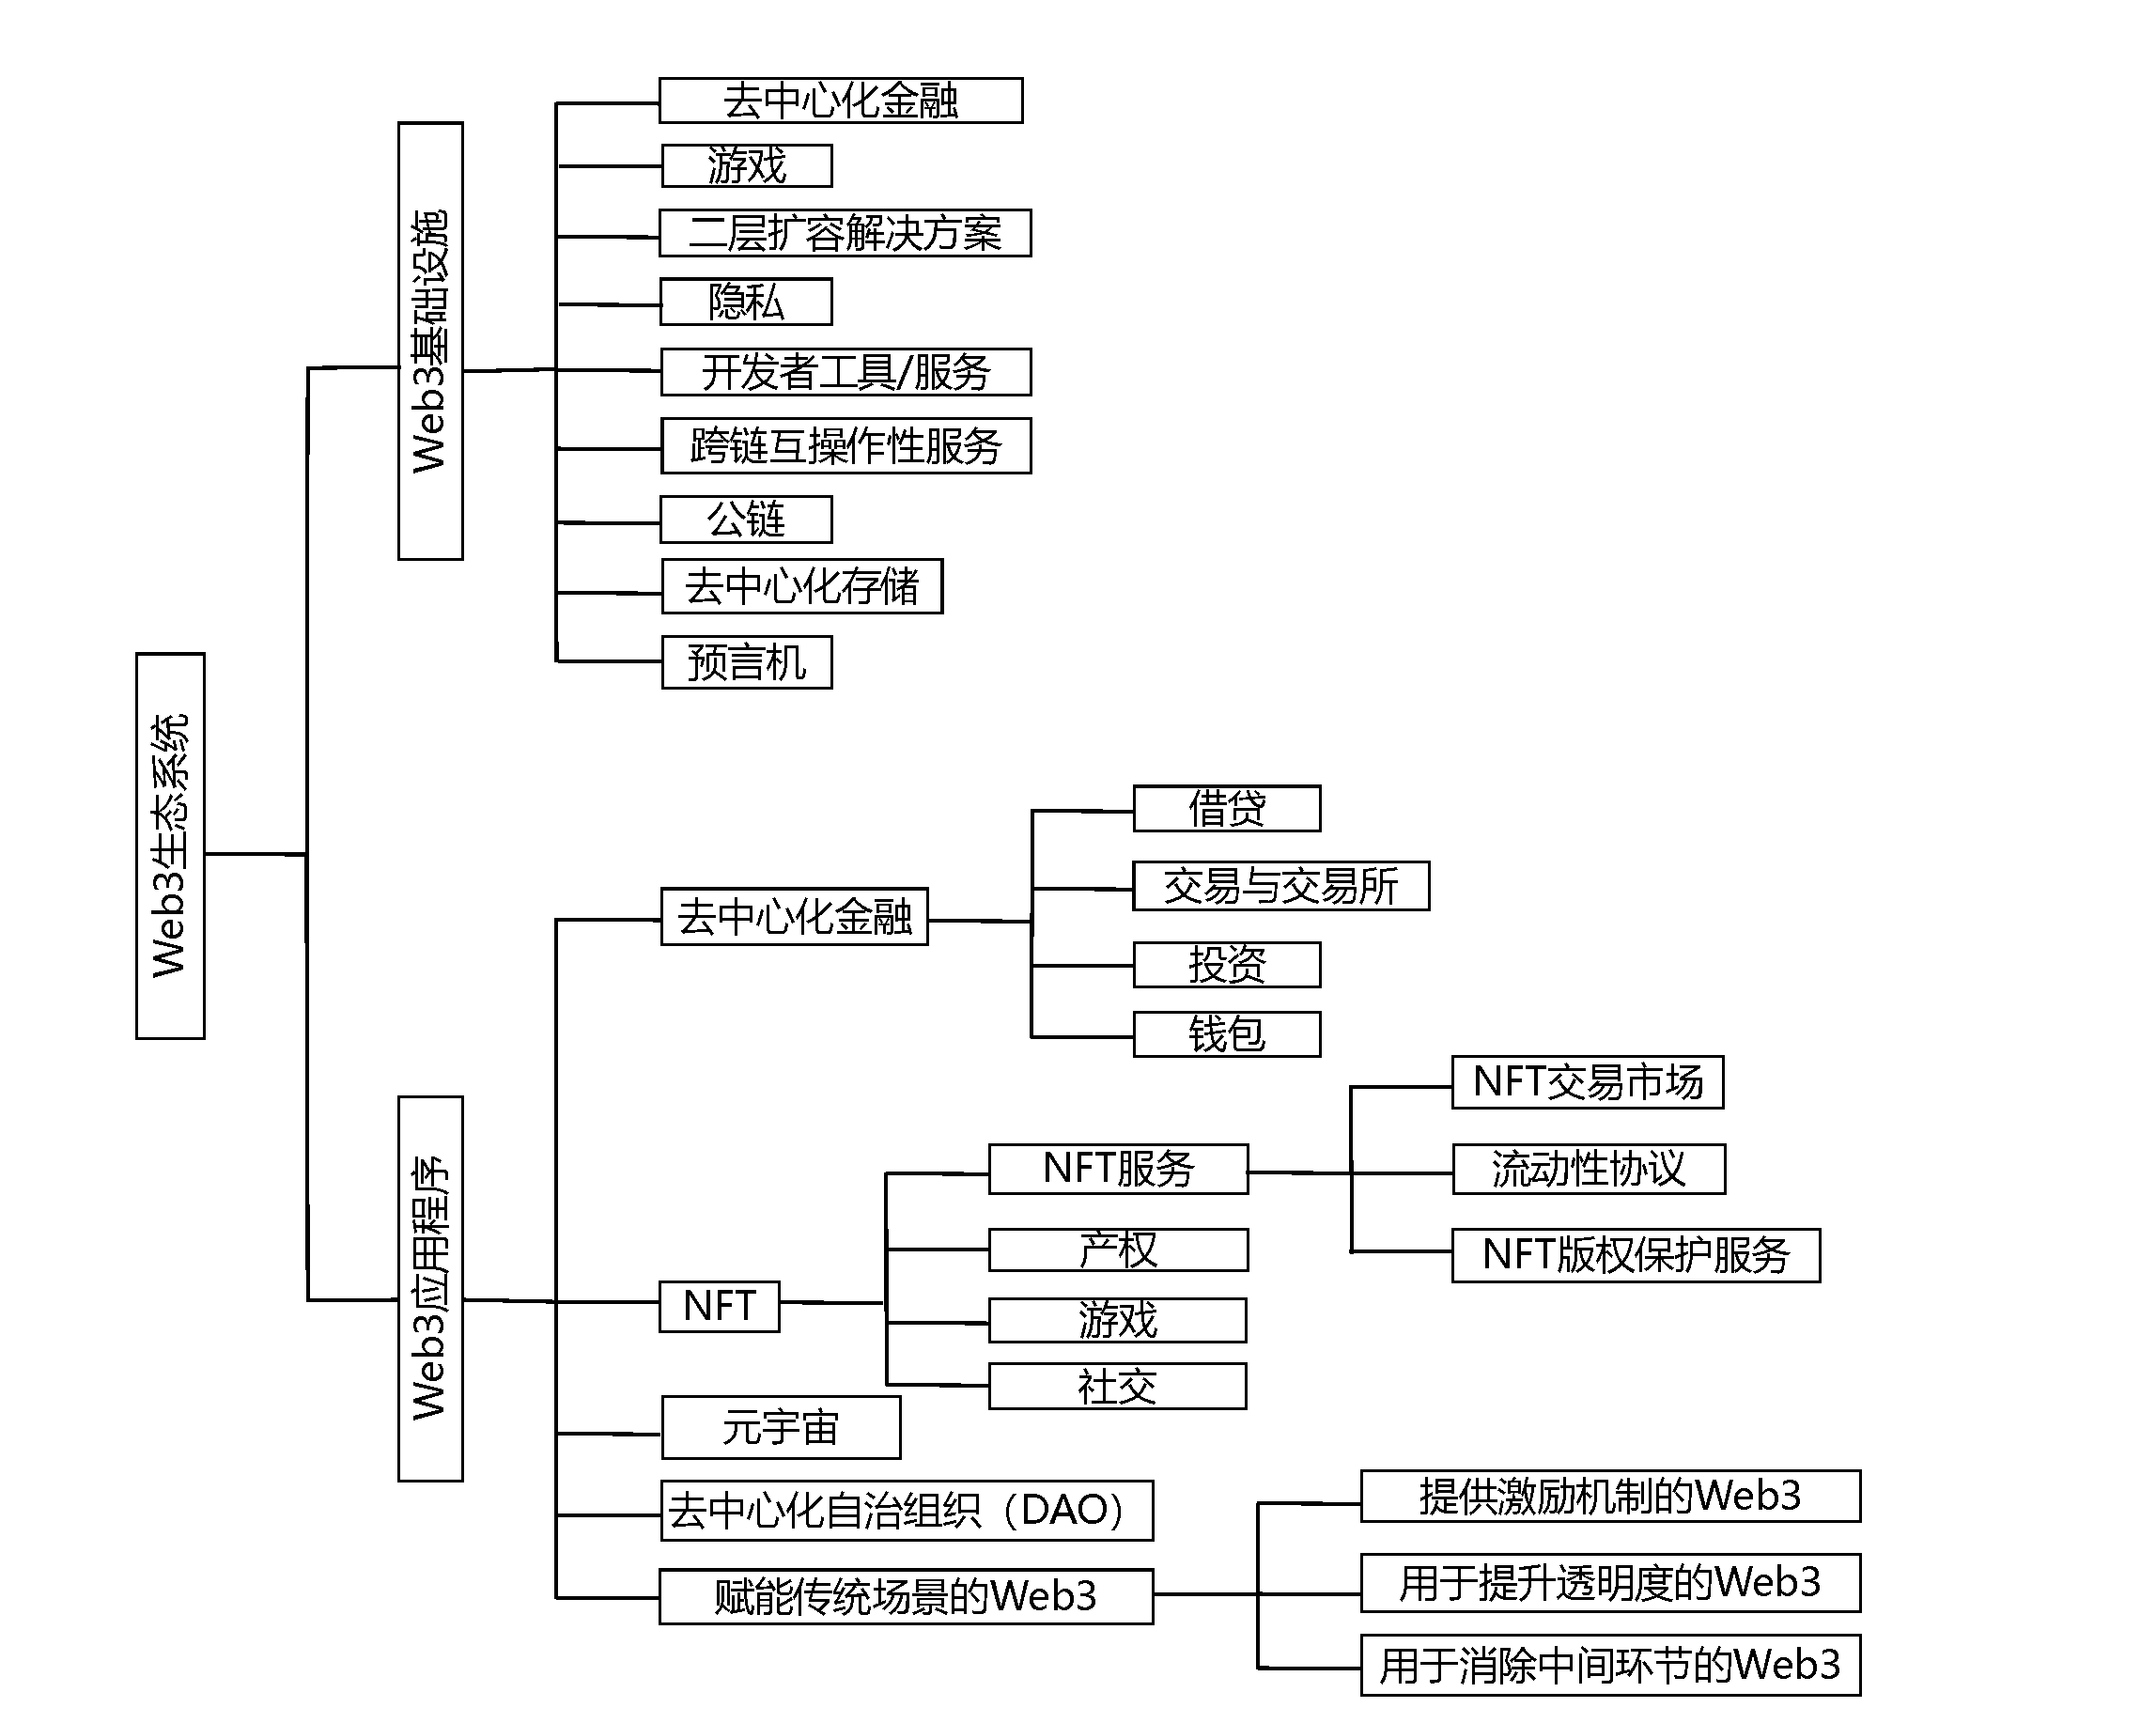
\includegraphics[width=1.1\linewidth]{./figures/web3_ecosystem.pdf} 
    \caption{Web3生态系统}
    \label{Fig:web3ecosystem}
\end{figure}


\subsection{Web3基础设施}
Web3基础设施涵盖了各种为开发者提供开发支持并增强区块链网络功能的解决方案。我们的分析确定了Web3基础设施的九个子类：去中心化金融~\cite{jensen2021introduction}基础设施、游戏基础设施、二层扩容解决方案~\cite{sguanci2021layer}、隐私基础设施、开发者工具/服务、跨链互操作性服务~\cite{pillai2020cross}、公链、去中心化存储~\cite{benisi2020blockchain}以及预言机~\cite{pasdar2023connect}服务。接下来，我们将详细介绍每一个子类，以及子类中有代表性的Web3项目。


\textbf{1.去中心化金融基础设施}

去中心化金融基础设施通过提供标准化的API或软件开发工具包来简化代币兑换功能的开发流程。

在去中心化金融基础设施领域，0x是一个具有代表性的项目~\cite{0x}。该项目在以太坊及多个兼容以太坊虚拟机的区块链上部署了支持ERC-20代币兑换的智能合约~\cite{erc-20}，这些合约能够聚合来自诸如Uniswap等去中心化交易所的流动性~\cite{uniswap, malamud2017decentralized}。此外，0x协议向开发者提供了用于实现代币兑换功能的标准化API，使其能够便捷地将该功能集成至Web3应用中，并共享来自多个交易平台的聚合流动性。


\textbf{2.游戏基础设施}

游戏基础设施能够协助缺乏区块链经验的开发者，将游戏内虚拟资产有效整合至区块链系统中。

Enjin~\cite{enjin}是该领域内具有代表性的项目之一，它支持开发者使用C/C++、Java和Python等主流编程语言进行游戏开发。通过Enjin，开发者可以创建虚拟资产，并为其分配相应的链上代币。Enjin提供的API接口使得这些代币能够顺利集成进游戏系统中。此外，Enjin还负责接收并监控来自游戏的相关请求，在区块链上完成处理后将结果返回游戏，实现链上链下的无缝对接


\textbf{3.二层扩容解决方案}

区块链网络吞吐量有限，成为制约Web3应用大规模部署的关键瓶颈。二层扩容方案在不修改底层协议的前提下提升网络处理能力，常见方法是在链下执行交易，仅将精简后的摘要信息上传至主链，从而缓解主链负载。

Optimistic Rollups是其中的典型代表，已被如Optimism~\cite{optimism}等以太坊虚拟机兼容网络广泛采用。该方案在二层打包并压缩多笔交易，默认其有效后统一提交至主链~\cite{schaffner2021scaling, chauhan2018blockchain}。任何节点在发现可疑交易时可提出欺诈证明发起挑战，验证失败将触发惩罚机制。该设计在提升系统吞吐量的同时维持了交易的正确性与网络的安全性。


\textbf{4.隐私基础设施}

在大多数区块链网络中，用户数据是公开可见的，这对用户隐私构成了挑战。隐私基础设施的核心在于防止交易记录暴露，降低用户身份与行为关联的风险。

Aztec Protocol~\cite{aztec}是典型的隐私基础设施之一，由一个以太坊智能合约和一个基于零知识证明技术的二层网络构成~\cite{sun2021survey}。用户将代币存入其智能合约后，资产被转移至Aztec的二层网络。在该网络中，用户可以私下转账或与接入Aztec的一层智能合约进行交互。所有交易以零知识简洁非交互式知识论证~\cite{petkus2019and}的形式表示，有效避免交易数据泄露。交易随后被打包并提交至以太坊主链。开发者可调用Aztec提供的API，将其智能合约与该协议集成，使Web3应用支持用户隐私交互。


\textbf{5.开发者工具/服务}

开发者工具和服务用于支持智能合约的开发、测试、部署与管理，提升开发效率并降低技术门槛。

ConsenSys~\cite{consensys}是该领域中广受采用的项目，旗下包括Infura~\cite{infura}和Truffle~\cite{truffle}等核心组件。Infura作为以太坊节点服务提供商，使开发者无需自建节点即可连接至以太坊网络，并提供账户管理、智能合约部署、交易签名与链上数据访问等API接口。Truffle则是一个完整的以太坊开发框架，涵盖合约编译、测试、部署以及交互式控制台功能，并配套提供用于Web3应用开发的相关库，构成高效的开发环境。


\textbf{6.跨链互操作}

区块链之间缺乏原生通信机制，导致数据与价值在多链环境中的流动受到限制。跨链互操作解决方案用于打通这一隔阂，支持不同区块链系统间的信息与资产交互。

Axelar~\cite{axelar}是该领域中应用广泛的代表，其作为一个独立的去中心化网络运行，拥有专属验证节点。该网络在连接的各条区块链上部署智能合约，形成互操作桥梁。合约由采用多方密码学的共享密钥控制，密钥被拆分并分配给各验证节点，持有份额与其质押的Axelar代币数量挂钩。验证节点在目标链上运行全节点，负责监测链上活动。当检测到用户向Axelar合约存入资产时，节点对跨链转移请求进行审批；一旦共享密钥中超过半数份额同意，合约即执行跨链转账操作。


\textbf{7.公链}

公链在设计上面临区块链不可能三角的结构性挑战~\cite{monte2020scaling}，即难以在去中心化、可扩展性与安全性三者之间同时取得平衡。

为在保证安全性的前提下提升可扩展性，多个公链正探索技术路径。NEAR~\cite{near}是一个具有代表性的项目，它提出通过名为Nightshade~\cite{skidanov2019nightshade}的分片技术~\cite{wang2019sok}来提高可扩展性。在该技术中，每个区块根据分片数量被拆分为多个数据块，由不同分片分别处理。网络通过可验证随机函数~\cite{micali1999verifiable}将各分片分配给部分验证节点。每个节点仅需存储并验证对应分片的数据块，而非完整区块，从而显著降低资源消耗，增强系统可扩展性。


\textbf{8.去中心化存储}

在以太坊等主流区块链网络中，数据需在所有节点上同步存储，导致存储成本显著上升。为缓解这一问题，去中心化存储网络应运而生，其运行机制在结构上与区块链相似。用户文件经过加密后分布式存储于网络节点，仅加密元数据（如文件位置和哈希值）被写入链上，从而避免将完整文件纳入区块，降低了成本。

Filecoin~\cite{filecoin}是建立在星际文件系统（IPFS）协议~\cite{benet2014ipfs}基础上的代表性项目。在该网络中，用户依据文件大小和存储时长支付费用，文件随后被分配至多个存储节点。为证明文件在约定时间内持续存在且未被篡改，节点需提交由文件生成的时空证明~\cite{moran2016proofs}与复制证明~\cite{benet2017proof}，以确保存储过程的可验证性和完整性。


\textbf{9.预言机}

预言机（Oracle）作为链下与链上之间的接口，用于将外部数据引入区块链，供智能合约调用。然而，若引入的数据无效或具恶意，可能对合约执行及用户资产构成威胁。

Razor Network~\cite{razor}提出一套激励与惩罚机制以提升数据可信度。数据提供者需质押代币作为担保，提交有效数据可获得奖励，提交无效数据则面临惩罚。这一机制强化了数据提供的诚实性，有助于保障智能合约运行的正确性及用户资产的安全性。


\subsection{Web3应用程序}
Web3应用程序是一类面向用户构建的去中心化应用集合。在本研究中，Web3应用被划分为五个子类别：去中心化金融（DeFi）、非同质化代币（NFT）、元宇宙、去中心化自治组织（DAO），以及面向传统场景的Web3应用。其中，DeFi、NFT与传统场景应用内部还包含多个细分类型，以下将分别展开论述。


\textbf{1.去中心化金融}

去中心化金融指的是运行在区块链之上的去中心化金融系统。在我们的数据集中，去中心化金融子类进一步细分为四个更小的子类：\textbf{i.借贷；ii.交易与交易所；iii.投资；以及 iv.钱包}。接下来，我们将对每个子类进行详细介绍。

\textbf{i.借贷。}借贷协议通过聚合多个贷方的资金，为借款方提供贷款服务，并从中收取利息作为贷方的收益来源。

Aave~\cite{aave}是该领域中的代表性协议，支持超额抵押借贷与闪电贷两类服务。在超额抵押借贷中，借款者需预先锁定价值高于贷款金额的加密资产作为抵押。若抵押资产价值跌破设定阈值，智能合约将自动发起清算流程，以回收资金并保障贷方利益。闪电贷~\cite{wang2020towards}面向具备编程能力的开发者，提供无需抵押的短时借贷。借款者需在单笔交易完成前偿还全部借款及利息，未按时偿还将导致交易整体回滚，确保资金安全。

\textbf{ii.交易与交易所。}
交易与交易所类应用程序主要包括一系列去中心化交易所，支持用户在链上进行代币兑换，无需依赖中心化托管方。而传统中心化交易所普遍采用订单簿机制~\cite{abudy2018corporate}，但在链上环境中，该模式通常效率较低，难以适应高频交易需求。

Uniswap是该领域的代表性项目，其采用自动做市商（AMM）算法~\cite{xu2021sok}替代传统订单簿机制。该算法基于流动性池运行，允许用户在无需等待撮合的情况下即时完成代币互换。兑换比例由池中两种代币的存量比例决定，遵循预设的定价函数，有效提升了交易效率与系统的去中心化程度。币兑换，使用户能够实现即时的代币互换。兑换比例是通过一种特定算法，根据池中两种代币的比例来确定的。

\textbf{iii.投资。}
投资协议在去中心化环境中承担类似投资基金的角色，将交易策略以代码形式嵌入智能合约中。用户将资金存入智能合约后，系统按照预设规则执行交易操作，产生的收益再按比例分配给用户。

TokenSets~\cite{tokensets}是该领域中应用广泛的协议，为用户提供多样化的投资组合。每个组合由一个智能合约管理，根据既定策略在去中心化交易所中对特定代币进行交易。该平台还支持用户自行定义投资策略并部署为智能合约，向其他用户公开，以实现策略共享与资产增值的双重目标。

\textbf{iv.钱包。}
钱包是用于管理加密资产并与Web3应用交互的工具，为用户提供账户控制与交易签名等功能。

MetaMask~\cite{metamask}是最为广泛使用的钱包之一，支持用户在多种设备上通过助记词创建或恢复以太坊账户，避免直接管理复杂的公私钥对。用户可使用MetaMask管理ERC-20代币，并与各类Web3应用无缝连接，完成资产转账、智能合约调用等操作。



\textbf{2.NFT}

NFT子类代表一类融合了非同质化代币元素的Web3应用~\cite{wang_non-fungible_2021}，可进一步划分为四个细分方向：\textbf{i. NFT服务；ii. 产权；iii. 游戏；iv. 社交}。以下将分别对各子类别进行详细介绍。

\textbf{i.NFT服务。}该方向包含以下三个更小的子类：\textbf{a.NFT交易市场；b.流动性协议；c.NFT版权保护服务}。


\textbf{a.NFT交易市场。}
NFT交易市场是专门用于非同质化代币买卖的平台。

OpenSea~\cite{OpenSea}是当前规模最大的NFT交易市场，支持用户交易多种类型的NFT资产，包括艺术品、音乐和游戏道具等。平台还提供铸造功能，允许用户在不具备区块链技术背景的情况下生成并发布自己的NFT。
	
    
\textbf{b.流动性协议。}
NFT通常价格较高，且存在流动性不足的问题。

为应对这一挑战，fractional.art~\cite{fractional}提出了基于所有权分割的流动性提升方案。该方法将NFT锁定在平台提供的智能合约中，并基于该资产发行多个ERC-20代币，每个代币对应NFT的一定比例所有权。此机制在保持资产完整性的同时，降低了投资门槛，有助于提升NFT的市场流动性。
	
    
\textbf{c.NFT版权保护。}
NFT市场频繁遭遇假冒问题，恶意用户常通过上传知名NFT的图像并重新铸造新NFT进行挂牌销售，扰乱市场秩序并侵犯原始作品版权。

Doppel~\cite{doppel}项目针对这一问题提出检测机制，利用计算机视觉与人工智能模型识别假冒NFT，并支持用户进行举报。目前，该系统已覆盖以太坊、Solana和波场等多个区块链平台，为NFT版权保护提供技术支持。


\textbf{ii.产权。}
NFT已被用于数字和实体产权的标识与保护。

在数字产权领域，Royal.io~\cite{Royal}提供基于NFT的音乐版权管理服务。艺术家可在平台上为其作品铸造NFT，并将歌曲名称、哈希值及版税分配比例嵌入至元数据中。当歌曲被他方使用或购买时，NFT持有者可按设定比例获得相应版税收益。在实体资产方面，Origyn~\cite{origyn}将实物资产（如手袋、手表与珠宝）的高清图像铸造成NFT，用作所有权凭证，从而在链上确权实体资产。


\textbf{iii.游戏。}
NFT技术已在游戏行业中得到应用，游戏内虚拟资产被铸造成NFT，使玩家重新获得对游戏数据的所有权。这类融合资产机制的游戏通常被称为“游戏化金融”，玩家在参与过程中有机会获得经济收益。

Axie Infinity~\cite{noauthor_axie_nodate}是该领域具有代表性的项目，玩家可在其中收集、繁育、饲养并交易虚拟宠物。每个宠物以NFT形式存在于区块链上，具备独立的所有权和市场价值。玩家既可以操控宠物参与对战，也可以将其出售以获取通证奖励，实现游戏与收益的结合。


\textbf{iv.社交。}
NFT技术已延伸至社交领域，为用户提供在不依赖中心化平台控制的前提下进行自我表达的手段。

Mirror~\cite{mirror}是该子类中的代表性项目，作为去中心化博客平台，允许用户发布内容并将其铸造成NFT。内容被存储在星际文件系统上，从而避免因平台干预导致的数据篡改或删除。用户还可购买创作者发行的NFT，以表达支持并参与内容生态的构建。

\textbf{3.元宇宙}

元宇宙~\cite{gadekallu2022blockchain}指由计算机系统构建的虚拟空间，可与现实世界交互融合，形成持续存在的数字环境。

许多元宇宙项目以区块链为基础，特点是在虚拟世界中将角色或资产铸造成非同质化代币（NFT）。The Sandbox~\cite{thesanbox}是面向虚拟地产的代表性项目，用户可在平台地图上购买土地并进行自主开发。这些土地以NFT形式记录在区块链上，具备明确的所有权，同时用户还可自由访问和浏览他人所构建的虚拟空间。 


\textbf{4.去中心化自治组织}

DAO（去中心化自治组织）~\cite{axelsen2023dao}是一种基于智能合约运行的组织形式，依靠预设规则自动执行治理与管理操作。

CreatorDAO~\cite{creatordao}是该领域的代表性项目，将投资者、创作者与支持者聚合于同一社区。该组织为创作者及其项目提供资金和资源支持，推动创作活动的发展。当作品产生收益时，智能合约依据既定规则自动完成利润分配，确保社区成员按其贡献获得相应回报。


\textbf{5.赋能传统场景的Web3}

Web3技术也已被许多传统行业所采用，以应对与激励机制、协作、透明度、信任等相关的挑战。基于Web3在传统行业中的功能，我们确定了三个子类别：\textbf{i.提供激励机制的Web3；ii.用于提升透明度的Web3；iii.用于消除中间环节的Web3}。


\textbf{i.提供激励机制的Web3。}
一些传统行业已开始在去中心化网络基础上开展业务，借此引入Web3提供的激励机制。

例如，Helium~\cite{helium}是一个基于区块链的无线网络运营平台。其向用户出售设备，用于提供网络覆盖和参与挖矿。用户部署设备后可获取通证奖励，作为其贡献网络资源的回报。该模式在降低企业基础设施建设和运营成本的同时，也使用户能够在传统通信场景中获得实际收益。


\textbf{ii.用于提升透明度的Web3。}
部分传统行业已引入Web3技术，将关键业务信息记录在区块链上，以增强透明度并解决信任问题。

Green Labs~\cite{greenlabs}和Blocery~\cite{blocery}为应用区块链于产品追溯的案例。它们将生产时间、流转路径和销售记录等核心数据上链，利用区块链公开、不可篡改的特性，实现从生产到销售全过程的可验证追溯。这一机制增强了信息透明度，有助于建立用户与企业之间的信任关系。


\textbf{iii.用于消除中间环节的Web3。}
Web3借助智能合约自动执行业务流程，省去了传统商业模式中对中介机构的依赖。

例如，Dtravel~\cite{dtravel}是部署在以太坊上的去中心化旅游平台，旅行者可直接与房产所有者通过智能合约完成预订，无需借助在线旅行社。该模式减少了中间环节，提高了交易效率与用户自主性。


\section{Web3代码和市场数据收集与分析}
本小节介绍了收集Web3项目中与代码和与市场相关数据的方法，以及相应的数据分析方法，以揭示Web3项目的流行度。

\subsection{代码和市场数据收集}
我们首先通过GitHub收集了Web3项目在Github的代码相关数据，然后通过Web3区块链浏览器（如Etherscan~\cite{etherscan}、Bscscan~\cite{bscscan}和Polygonscan~\cite{polygonscan}）收集了Web3项目的市场相关数据。

对于代码相关数据，我们首先人工检查Web3项目是否在GitHub上有开源代码库。在人工审查了200个Web3项目后，我们确定了96个开源的Web3项目。然后，我们通过爬虫收集了所确定的这96个项目在GitHub中的代码相关数据（代码行数和提交次数）。

对于市场相关数据，我们利用区块链浏览器的API获取了每个Web3项目在2022年1月至2023年1月期间的交易数和市值数据（包括市值和唯一钱包数）。


\subsection{代码层面的流行度分析}
对于Web3基础设施和Web3应用程序的每个子类，我们计算了开源项目的数量，以及所有项目的代码存储库的代码总行数和提交次数（见表~\ref{Table:githubdata}），这些数据用于从代码层面量化特定子类的流行度。项目数量更多、代码行数更多且提交次数更多的子类别被认为更受欢迎。

此外，我们分析了每个Web3项目所使用的编程语言以及部署的区块链平台。然后，我们总结了每种编程语言的使用频率以及部署在不同区块链平台上的Web3应用程序数量，以了解编程语言和区块链平台的流行度。


\begin{table}[!htbp]
\centering
\caption{Web3项目的代码相关数据}
\label{Table:githubdata}
\vspace*{-0.25cm}
\tabcolsep=16.5pt
\begin{tabular}{lcll}
\hline
\textbf{子类别} & \textbf{项目数量} & \textbf{代码行数} & \textbf{提交次数} \\
\hline
公链 & 17 & 3,386,348 & 124,040 \\

跨链互操作性 & 9 & 3,156,655 & 39,720  \\

开发者工具 & 8 & 641,749 & 11,998  \\

去中心化存储 & 7 & 421,291 & 17,708  \\

预言机 & 3 & 364,499 & 872  \\

游戏基础设施 & 2 & 309,826 & 6,330  \\

Layer 2 扩展方案 & 2 & 2,071,208 & 15,594  \\

隐私保护 & 2 & 436,352 & 7,960  \\

DeFi 基础设施 & 1 & 105,496 & 17,137  \\

借贷 & 12 & 595,999 & 11,205  \\

交易与兑换 & 7 & 214,912 & 2,756   \\

投资 & 4 & 80,193 & 2,919  \\

DAO & 1 & 2,793 & 55   \\

钱包 & 2 & 162,163 & 4,533  \\

NFT 市场 & 2 & 117,305 & 2,977  \\

NFT 流动性 & 2 & 56,843 & 454  \\

NFT版权保护 & 1 & 14,091 & 3 \\

产权类 & 2 & 105,070 & 806  \\

游戏 & 3 & 28,002 & 162   \\

元宇宙 & 1 & 462,462 & 5,656  \\

提供激励机制的Web3 & 2 & 98,049 & 3,804 \\

消除中间环节的Web3 & 4 & 20,992 & 321  \\
\hline
\end{tabular}
\vspace*{-0.5cm}
\end{table}





\begin{table}[!htb]
\centering
\caption{Web3项目的市场相关数据}\vspace*{-0.25cm}
\tabcolsep=14.5pt
\begin{tabular}{llll}
\hline
\textbf{子类别} & \textbf{项目数量} & \textbf{用户数} & \textbf{市值} \\
\hline
借贷 & 14 & 129,188 & \$1,827,265,578   \\

交易与兑换 & 11 & 843,178 & \$5,831,446,783  \\

投资 & 2 & 22,287 & \$2,682,758,809 \\

NFT 市场 & 4 & 2,070,447 & \$24,687,589,059  \\

产权类 & 4 & 16,422 & \$28,864,897  \\

游戏 & 17 & 193,249 & \$1,249,040,083  \\

社交 & 3 & 18,780 & \$8,753,611  \\

元宇宙 & 1 & 220,532 & \$950,498,005  \\

DAO & 4 & 49,375 & \$1,177,325,522   \\

提供激励机制的Web3 & 3 & 477,043 & \$522,377,779  \\

消除中间环节的Web3 & 2 & 2,910 & \$16,049,029 \\

\hline
\label{Table:marketdata}
\end{tabular}
\end{table}



\subsection{市场层面的流行度分析}
我们将Web3项目划分为两组：一组部署在多个区块链平台上，另一组仅部署在单一平台上。每组均包含项目名称、用户数量及市值数据。通过比较两组的用户数量中位数和市值中位数，并参考其最大值，评估部署在多个平台与单个平台之间在用户覆盖和市值表现上的差异。

采用相同方法，将Web3项目进一步划分为开源与非开源两类，并分别计算其用户数量和市值的中位数与最大值，以分析开源策略对项目影响的具体体现。

此外，针对Web3项目的各个子类，统计了每类应用的用户总数与总市值（见表~\ref{Table:marketdata}），以从市场维度衡量其受欢迎程度。最后，对各Web3应用的用户数量进行了分布分析，图~\ref{Fig:uaws}展示了相关统计结果。


\section{Web3项目的流行度}
本小节从代码层面与市场层面分析了Web3项目的流行度，相关结果有助于从业者与研究人员识别Web3生态中的开发者偏好与技术趋势，以及了解用户对不同类型应用的接受程度及其不同类型应用的市场价值。


\subsection{代码层面的流行度}
代码层面的研究结果揭示了开发者偏好与项目流行度之间的关系，反映出不同类型Web3基础设施与应用在开发实践中的受关注程度，以及开发者在部署平台选择上的倾向。

表~\ref{Table:githubdata}汇总了Web3项目的代码相关数据，首列列示了开源项目的子类别，其中第1至第9行对应Web3基础设施，第10至第21行对应Web3应用。图~\ref{Fig:platformdistribution}进一步展示了这些项目在各区块链平台上的分布情况。基于表中数据，可归纳出以下观察发现：

 \begin{figure}[!htbp]
 \centering
		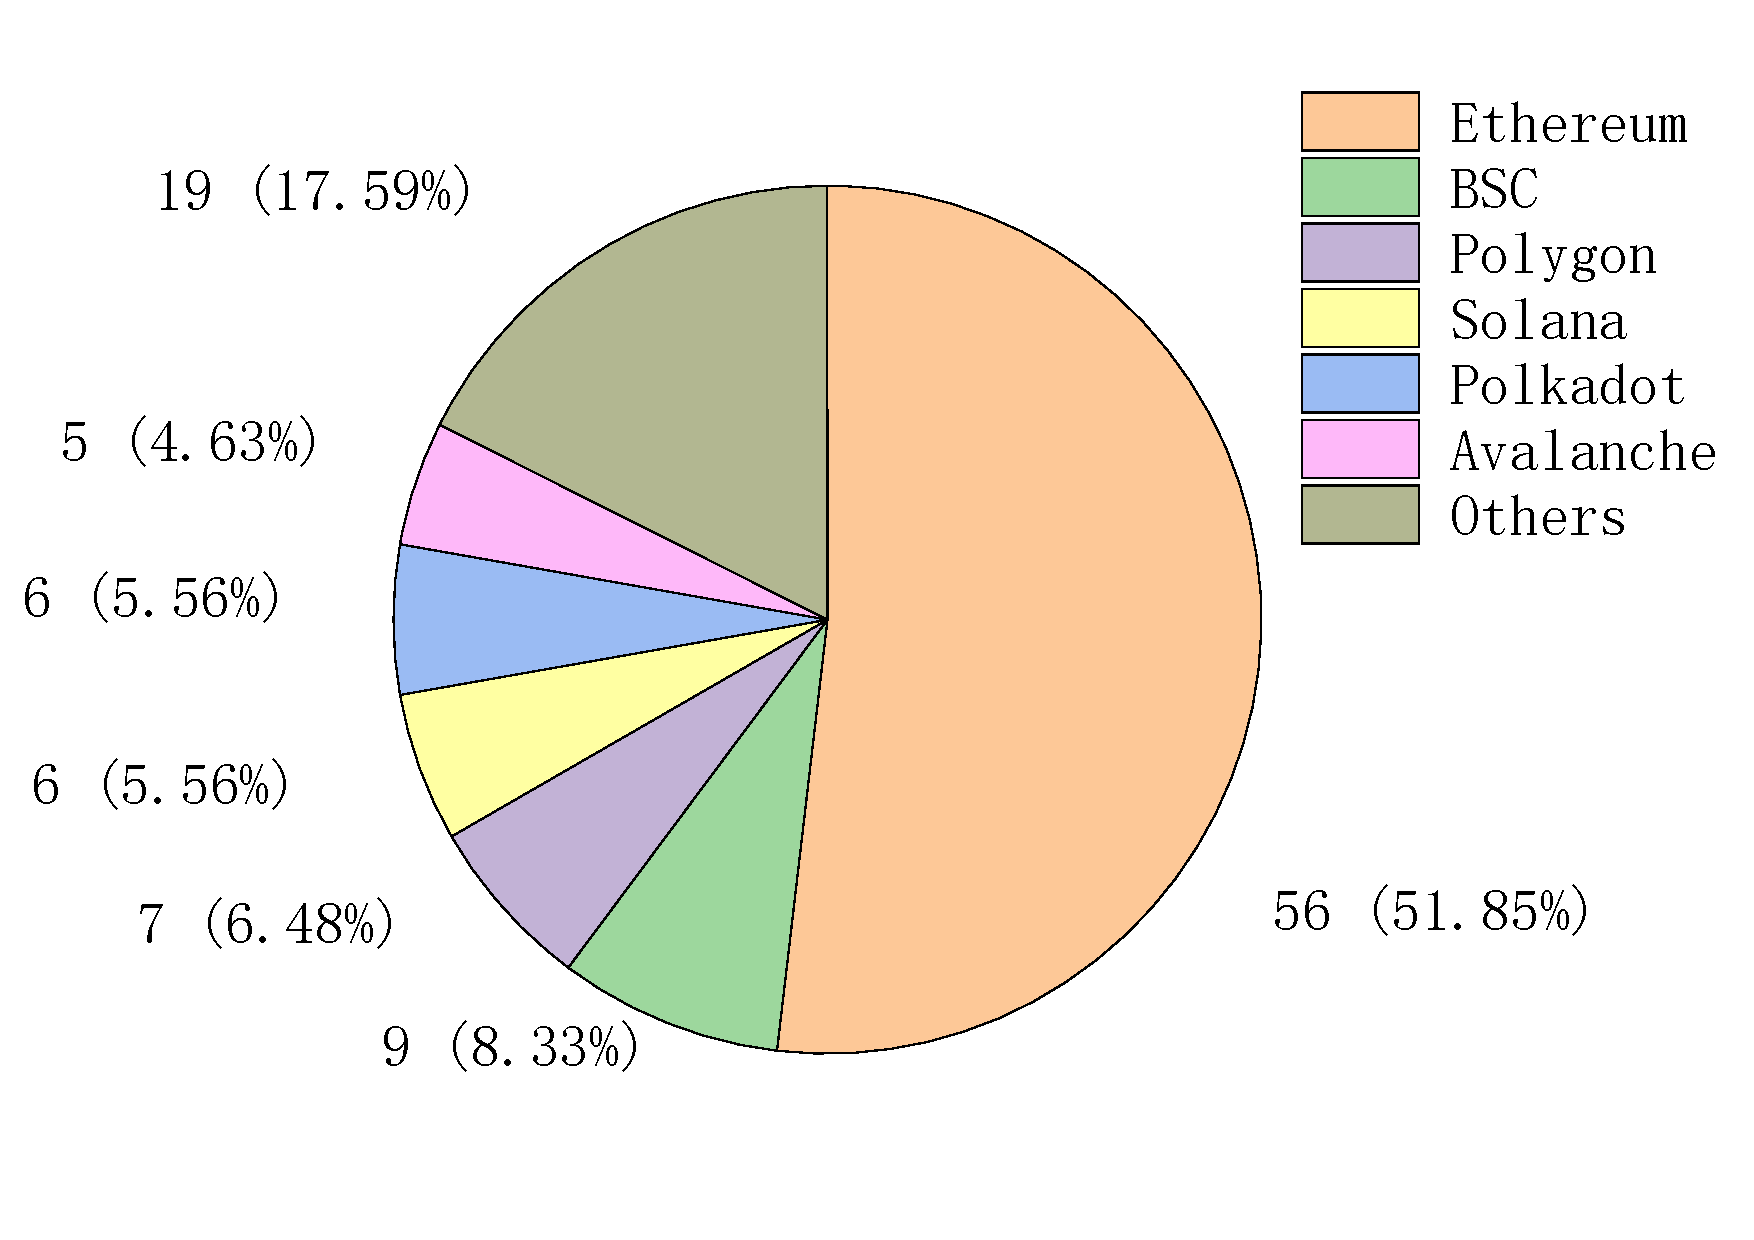
\includegraphics[width=0.6\textwidth]{./figures/platform2.pdf} 
        \vspace*{0.25cm}
		\caption {Web3项目在不同区块链网络的分布} 
		\label{Fig:platformdistribution}
\end{figure} 


\textbf{1. 公链在Web3基础设施中具有最高的开发活跃度。}

如表~\ref{Table:githubdata}所示，开源Web3基础设施项目中，公链类项目数量最多，共17个。此外，该类别在代码行数（3,386,348行）和提交次数（124,040次）方面排名最高，反映出其在开发者中的开发活积极性最高。

\textbf{2. 借贷类应用在Web3应用开发中表现出最高活跃度。}

根据表~\ref{Table:githubdata}，在Web3应用的各子类别中，借贷类项目的开源数量为12个，为数量最多的一类。同时，该类别的代码行数为595,999行，提交次数为11,205次，均高于其他子类别，显示出该领域在开发中的活跃程度最高。


\textbf{3.以太坊是部署Web3应用最主要的网络。}

如图~\ref{Fig:platformdistribution}所示，在108个Web3应用中，56个部署在以太坊网络，占比51.85\%。相比之下，其他区块链网络上的Web3应用数量在5至19之间，占比介于4.63\%至17.59\%。该数据表明，以太坊在智能合约部署方面具有较强的吸引力。



\textbf{4.Solidity~\cite{dannen2017solidity}是智能合约开发中最广泛使用的编程语言。}\label{solidity_37}

在41个开源Web3应用中，有37个采用Solidity作为智能合约开发语言，表明该语言在Web3应用开发中受到开发者的广泛青睐。



\subsection{市场层面的流行度}
市场层面的研究结果揭示了Web3应用在用户活跃度和市场认可度方面的表现。这些发现有助于识别用户规模较大、市值水平较高的应用特征，并分析在Web3生态中较受欢迎的活动类型及其用户增长趋势。

图~\ref{Fig:2-1}展示了Web3应用的用户数量与市值分布情况，图~\ref{Fig:uaws}呈现了2022年1月至2023年1月期间的用户增长曲线。表~\ref{Table:marketdata}则汇总了各项目的市场数据。基于上述信息，可得出以下观察发现：

\textbf{1.多链部署的Web3应用拥有更多用户和更高市值。}

如图~\ref{Fig:2-1}(a)所示，第一个和第二个箱形图分别展示了多链部署与单链部署Web3应用的市值分布。多链部署应用的市值中位数和最大值均高于单链部署，反映出其在市场价值层面的相对优势。

类似趋势也体现在用户数量上。图~\ref{Fig:2-1}(b)中的箱形图对比了两类部署方式下的用户数量分布，多链部署的应用在中位数和最大值上均优于单链部署，表明其用户覆盖范围更广，活跃度更高。

\begin{figure}[!htbp]
\centering
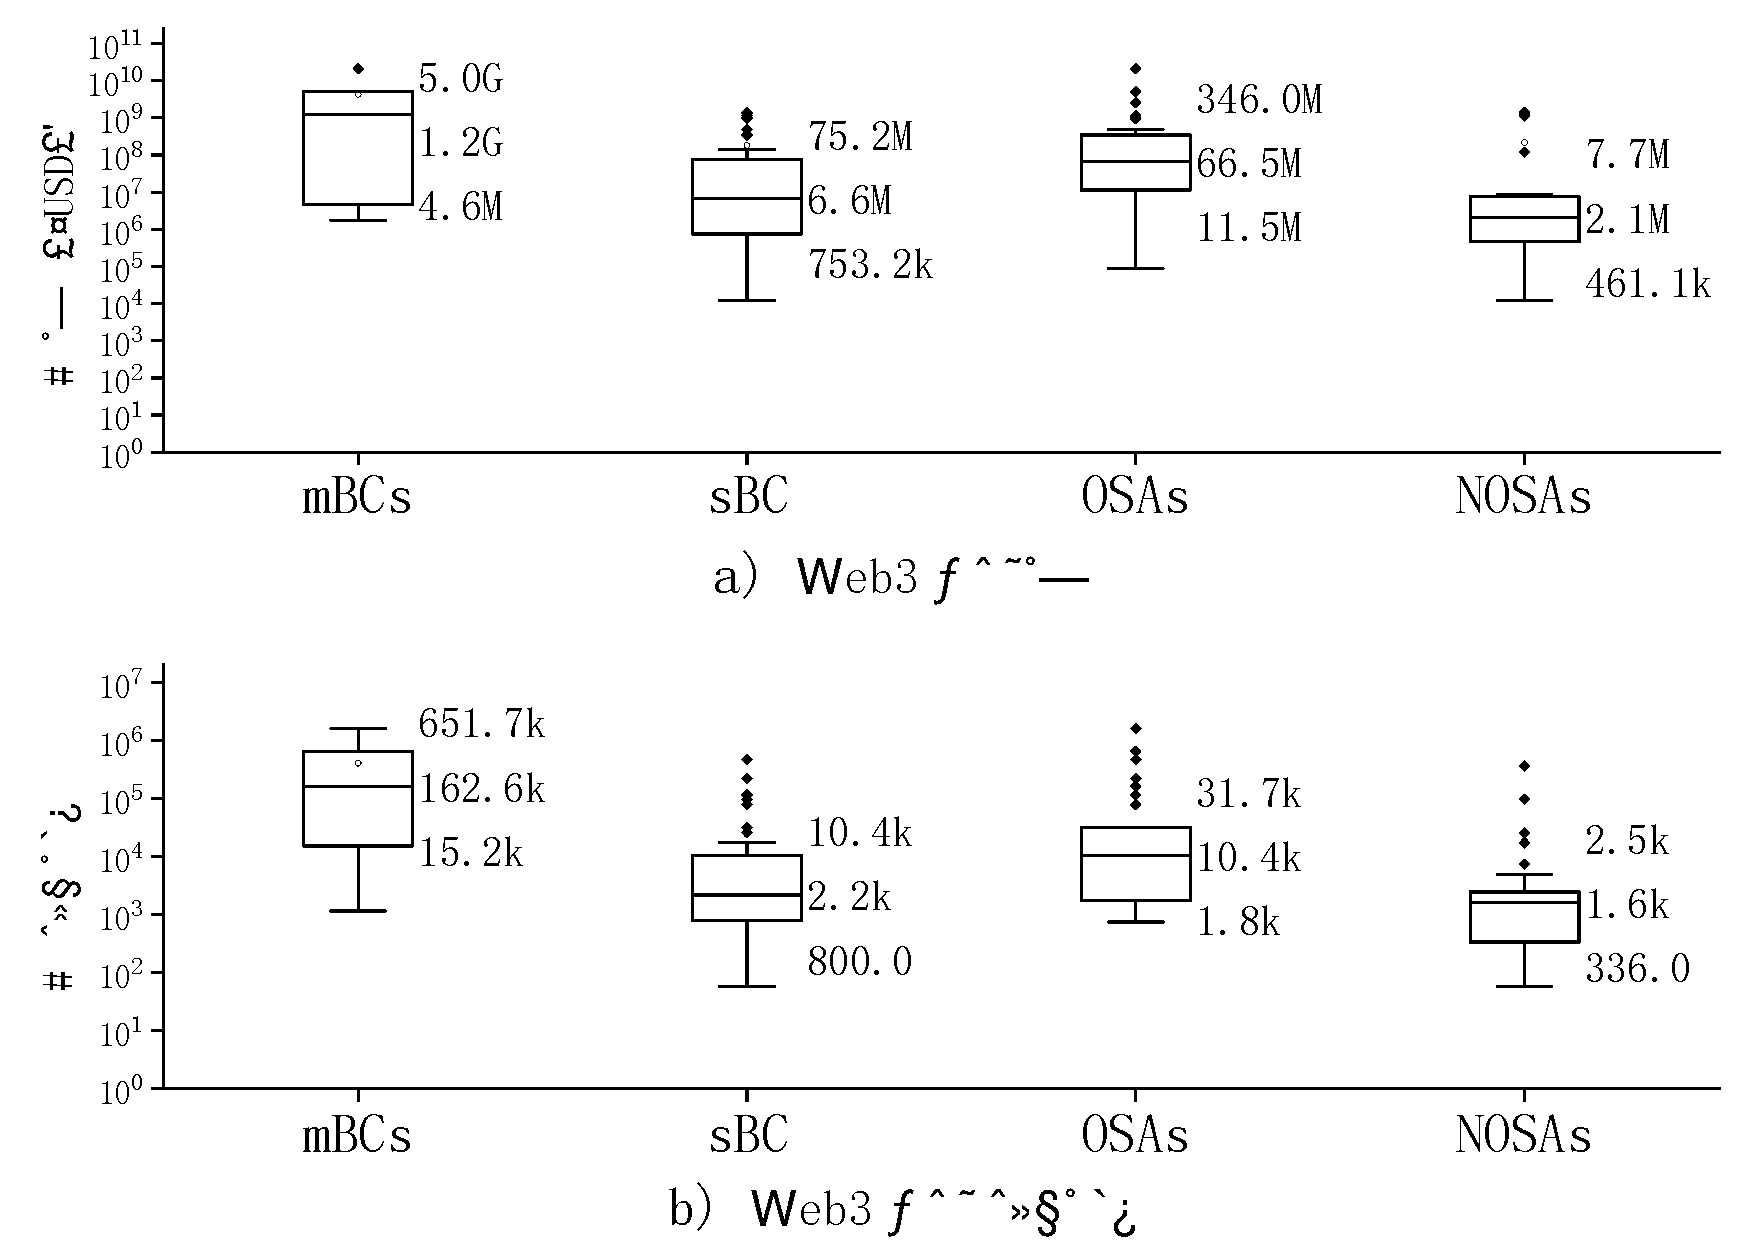
\includegraphics[width=0.8\textwidth]{./figures/2-1.pdf} 
\caption[用户数量与市值的分布情况]{用户数量与市值的分布情况。\textbf{mBCs}表示多链部署的应用程序。\textbf{sBC}表示单链部署的应用程序。\textbf{OSAs}表示开源应用程序，而\textbf{NOSAs}表示非开源应用程序。}
\label{Fig:2-1}
\end{figure}




\begin{figure}[!htbp]
\centering
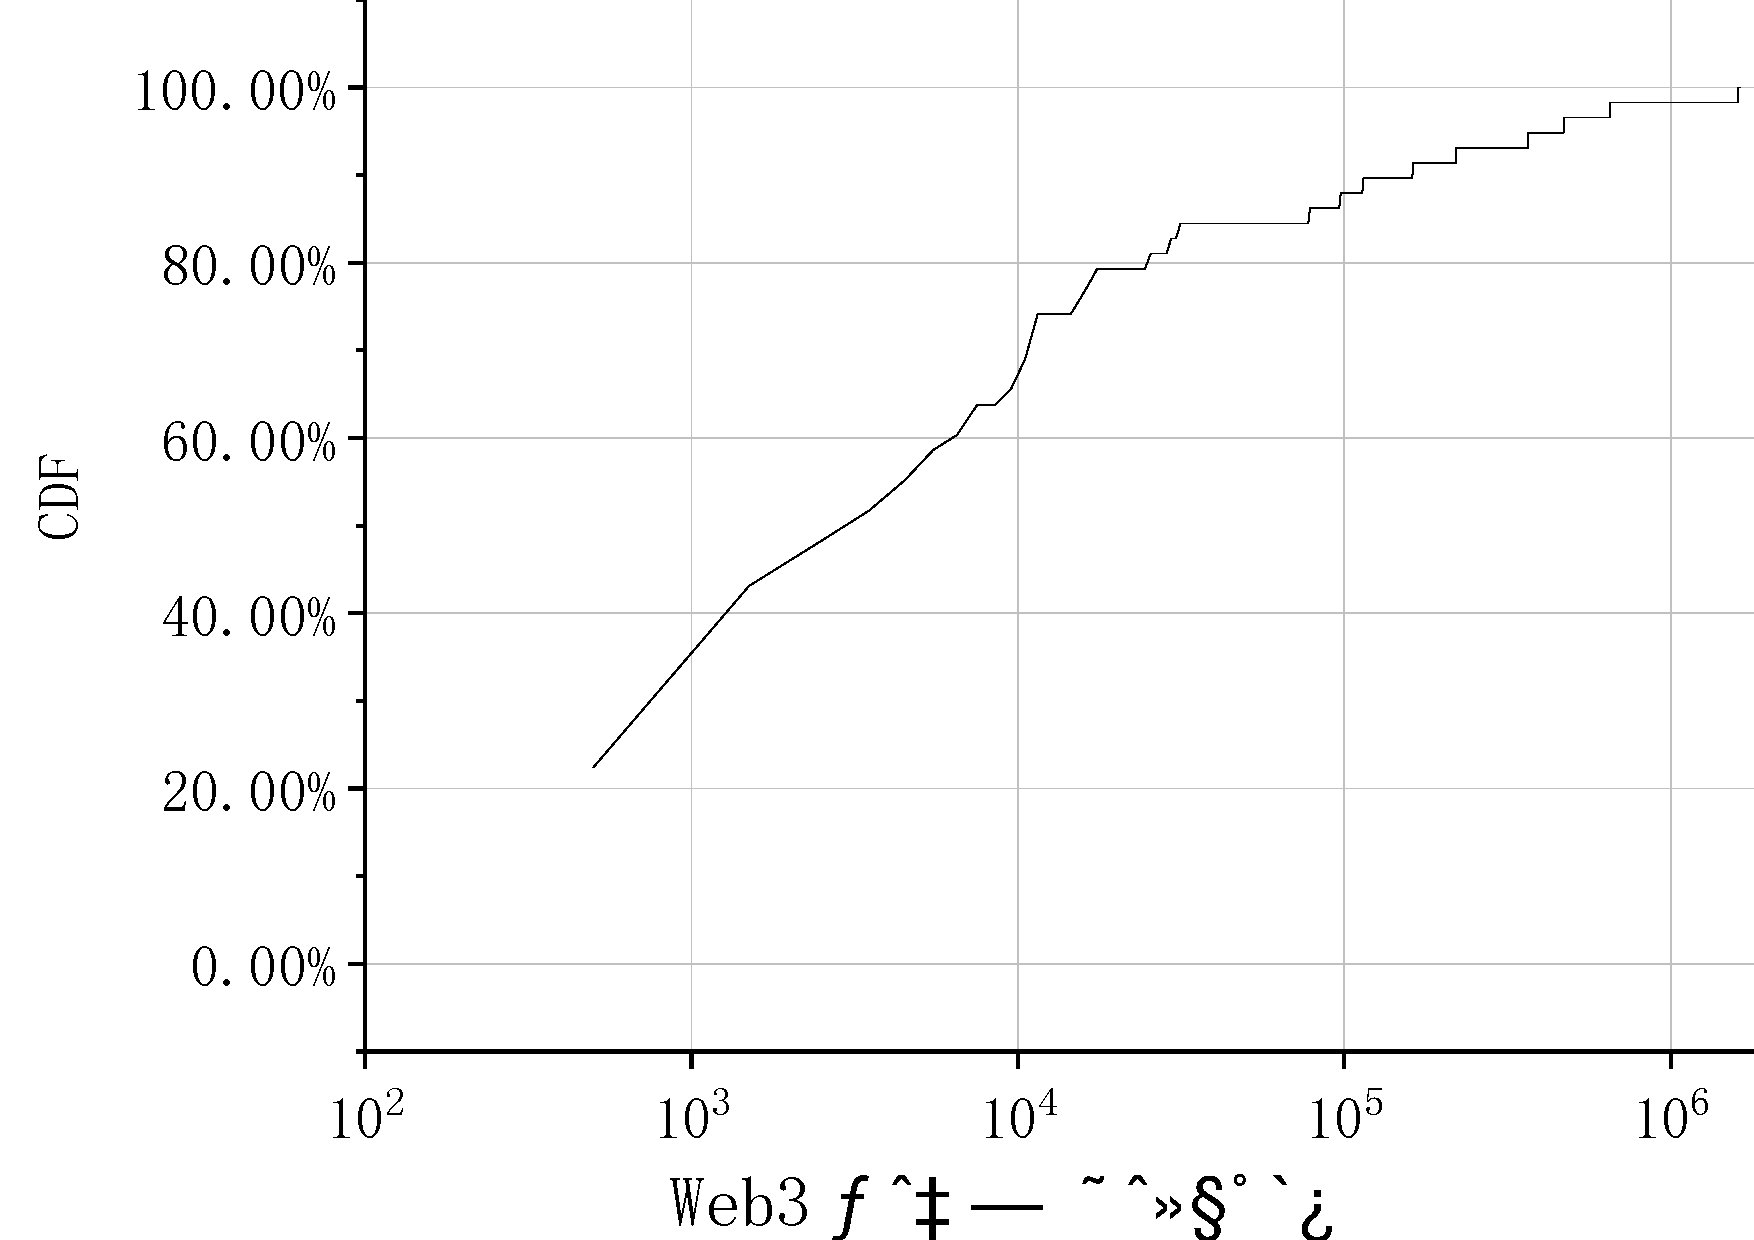
\includegraphics[width=0.6\textwidth]{./figures/uaws.pdf} 
\caption[Web3应用程序的用户数量]{2022年1月到2023年1月期间Web3应用程序的用户数量。}
\label{Fig:uaws}
\end{figure}







\textbf{2.开源Web3应用在用户吸引力和市值方面表现更为突出。}

图~\ref{Fig:2-1}(a)中的第三与第四个箱形图分别展示了开源与非开源Web3应用的市值分布。结果显示，开源应用的市值中位数和最大值均高于非开源项目。这一差异可能反映出开源带来的透明度、社区参与度以及用户信任水平在提升市场认可度方面的积极作用。

图~\ref{Fig:2-1}(b)进一步呈现了两类项目的用户数量分布。开源应用的用户数量最大值显著高于非开源应用，后者的用户数量中位数相对较低，表明开源项目在用户层面具备更强的吸引力和增长潜力。


\textbf{3.NFT交易是Web3生态系统中用户最活跃的子类。}

如表~\ref{Table:marketdata}所示，NFT市场的用户数量为2,070,447，位居各应用类别之首，其市值也达到24,687,589,059美元，处于较高水平。这一结果表明，NFT交易是Web3中最受用户欢迎的应用。



\textbf{4.约65\%的流行Web3应用在2022年至2023年期间用户增长数未超过10,000。}
图~\ref{Fig:uaws}展示了2022年1月至2023年1月期间，热门Web3应用累计独立用户数量的累积分布函数。数据显示，大约65\%的应用在一年内的新增用户数量未超过10,000。这一趋势揭示了Web3在用户获取上的挑战，同时也体现了该领域整体仍处于发展初期。


\section{Web3智能合约的问题报告收集与分析}
Web3问题报告是指开源Web3项目在Github的问题报告。本小节主要介绍通过Github收集Web3项目的问题报告方法，以及如何使用大语言模型分析这些问题报告，以便洞察和识别Web3中可能存在的漏洞及开发者对待漏洞的处理方式。


\subsection{Web3智能合约问题报告收集}
在本小节，我们首先筛选了175个包含问题报告的开源Web3项目仓库，然后开发了一款爬虫程序，从这些仓库中爬取了1175条问题报告。具体步骤如下。

\textbf{步骤一：识别包含问题报告的Web3项目仓库}

首先，我们从获得风险投资的200个Web3项目中筛选出23个在GitHub平台上包含问题报告的项目。然而，由于该数量较为有限，难以全面反映Web3领域的问题，因此，为了进一步扩大数据规模、提升问题报告的覆盖率，并确保所收集数据的广泛性和代表性，我们利用GitHub的高级搜索功能，以“Web3”为关键词进行检索，额外识别出152个包含问题报告的开源Web3项目仓库。

具体而言，我们开发了一款爬虫脚本，用于自动识别GitHub上包含问题报告的项目仓库。数据筛选过程包括以下几个步骤：

\textbf{1.关键词与筛选条件}：采用“Web3”作为核心关键词，并将Solidity设定为编程语言的筛选条件。Solidity的选取基于其在Web3智能合约开发中的广泛应用。在章节~\ref{solidity_37}的发现中显示：41个开源Web3应用中，有37个使用Solidity语言编写其后端智能合约。

\textbf{2.数据排序与筛选}：在搜索结果中，我们按照Star数量降序排列，并获取前100页的搜索结果（GitHub的搜索功能仅允许访问前100页的结果）。

\textbf{3.问题报告筛选}：在获取的GitHub仓库列表中，我们在项目链接后附加"/issues?q=is\%3Aissue"以筛选出包含问题报告的仓库。

经过上述筛选流程，我们最终确定了175个包含问题报告的Web3项目仓库。



\textbf{步骤二：收集问题报告}

在确定了包含问题报告的175个Web3项目仓库后，我们开发了一款自动化爬虫脚本，从这些仓库中收集到了1175个问题报告。
具体而言，对于每条问题报告，我们提取以下关键信息：

\textbf{标题}：问题报告的概述，通常由开发者对问题的简要描述。

\textbf{正文}：详细的错误信息，例如漏洞的描述或者漏洞代码。

\textbf{评论}：开发者针对问题的讨论、分析以及修复方案。

所有数据均以结构化JSON格式存储，每条记录包含title、body和comments三个核心字段，以便后续自动化分析与人工审查。

需要注意的是，在数据采集过程中，我们仅爬取了已关闭的问题报告，并过滤掉开放中的问题报告。此选择主要基于以下考虑：

1. 开放的问题报告仍处于讨论阶段，其中提及的漏洞尚未得到充分验证，可能包含大量不确定性信息。

2. 已关闭的问题报告通常包含更高质量的讨论，并附有开发者的反馈与完整的修复过程，从而有助于准确理解Web3项目中的常见问题及其解决方案。

最终，我们成功从175个Web3项目仓库中爬取了1175个问题报告。



\subsection{基于大语言模型分析问题报告}
在问题报告收集完成后，我们调用了大语言模型DeepSeek\_v3的API，并设计了一条结构化提示词对问题报告进行自动化分析。目的是高效识别漏洞相关问题、总结问题核心内容、对潜在漏洞进行分类以及归纳开发者对漏洞的讨论，具体提示词如图~\ref{fig:prompt-issue-analysis}所示。


\begin{figure}[H] 
\centering
\begin{tcolorbox}[
  enhanced,
  breakable=false,   
  colback=gray!10,
  colframe=black,
  boxrule=0.5pt,
  arc=0pt,
  left=5pt,
  right=5pt,
  top=5pt,
  bottom=5pt,
  title={问题报告分析提示词模板},
  fonttitle=\bfseries
]

\#\#\# Github 问题报告信息：

标题: \{title\}  

正文: \{body\}  

\#\#\# 请基于问题报告的标题和正文回答以下问题：  

1. 该问题是否涉及漏洞？  
2. 若涉及漏洞，总结该问题的核心内容。  
3. 若涉及漏洞，请分类漏洞类型（如整数溢出）。  

开发者回复: \{comments\}  

\#\#\# 请基于 comments 总结开发者的讨论内容，并用以下JSON格式返回结果：

\{
  "original issue": \{
    
    "title": "原始问题标题",
    
    "body": "原始问题描述",
    
    "comments": ["comment 1", "comment 2", "comment 3"]
    
  \},
  
  "analysis": \{
  
    "is vulnerability": true,
    
    "summary": "...",
    
    "vulnerability type": "...",
    
    "cause analysis": "...",
    
    "developer comments": "..."
          \}
\}
\end{tcolorbox}
\caption{问题报告分析提示词模板}
\label{fig:prompt-issue-analysis}
\end{figure}




根据该提示词，大模型将依次执行以下自动化分析流程。首先，大模型基于问题报告的标题与正文提取并概括核心讨论内容。在此基础上，模型判断问题是否涉及漏洞；若涉及漏洞，则进一步对漏洞进行分类（如整数溢出、DOS攻击等）。随后，模型基于开发者的评论归纳其讨论内容，包括修复方案与争议焦点。最终，模型以结构化的JSON格式输出分析结果，具体包含原始问题数据及分析结论。分析结论涵盖对问题报告的核心总结、是否涉及漏洞的判断、漏洞类型、漏洞产生的可能原因以及开发者对待漏洞的观点。

基于上述自动化分析流程，我们对1175条问题报告进行处理，成功识别出280条涉及漏洞的问题报告。下一节中将对这些问题报告及模型返回的分析结果进行人工审查，进一步探讨漏洞类型及开发者对待漏洞的处理方式与观点。



\section{Web3智能合约漏洞}
在本小节中，我们对280条漏洞报告进行了人工分析，详细审查了每条报告的结构化信息，包括漏洞概要、漏洞类型以及漏洞成因。通过系统性归纳分析，我们发现Web3领域的漏洞主要可分为以下两类：

\textbf{(1) 通用漏洞}

此类漏洞通常源于区块链底层机制或智能合约代码实现中的共性问题，适用范围广泛，并非特定于某个具体应用或合约。攻击者可将同一漏洞利用方式复用于多个项目或协议中，因此造成的安全风险较大，具有明显的通用性，例如典型的整数溢出漏洞。

\textbf{(2) 业务逻辑漏洞}

此类漏洞通常源于特定合约或协议在业务逻辑设计上的缺陷，仅在特定的运行流程或交互模式下才会被触发，难以在其他协议中复用，因此缺乏普遍适用性。
例如，在借贷平台Aave的一个关于业务逻辑漏洞的问题报告指出，该平台的还款流程中支持用户使用持有的存款凭证（即代表存入资产的代币）直接偿还债务。但在这一流程中，系统未对用户的健康因子进行校验，攻击者可借此在资金不足、健康因子过低的情况下清除自身债务，同时制造系统内的坏账，从而非法提取资金。由于该漏洞依赖于Aave协议特有的还款机制与债务模型，难以在其他协议中复现，因此不属于通用漏洞。


基于上述分类，我们将研究聚焦于可能影响多个Web3应用程序或智能合约、具有较广泛攻击面的通用漏洞上。经过系统分析，我们总结出以下八类常见的通用漏洞。


\textbf{1.访问控制漏洞}

合约在权限管理方面存在设计或实现缺陷，导致未授权用户能够调用受保护的合约函数。此类漏洞通常源于访问修饰符配置不当或逻辑判断缺失，可能导致关键操作被绕过，引发资产被非法操作或敏感状态被篡改的风险。

\textbf{2.不安全随机数漏洞}

合约依赖可预测的链上数据（如区块哈希、时间戳等）生成随机数。由于这些数据可被区块生产者或攻击者部分控制，随机性不足将影响系统的公平性与安全性，尤其在涉及博弈、抽奖等场景中易被利用。

\textbf{3.整数溢出漏洞}

当运算结果超出数据类型的表示范围而未被检测时，会导致整数溢出或下溢。这类漏洞常见于代币合约中，可能引起余额异常、计算错误等问题，进而造成资产损失或状态异常。


\textbf{4.重入攻击漏洞}

攻击者在外部调用过程中通过递归调用目标合约函数，在其状态更新完成前多次触发关键逻辑，从而操纵或窃取合约资产。此漏洞通常与以太币转账函数配合使用的外部调用有关，是经典且高危的攻击路径。

\textbf{5.区块信息依赖漏洞}

合约依赖区块信息（如时间戳）作为关键逻辑的输入时，可能被矿工或验证者利用对区块生产过程的控制进行操控，从而改变合约行为。该问题破坏了合约逻辑的确定性与安全性。

\textbf{6.拒绝服务攻击漏洞}

攻击者利用构造极高gas消耗的输入、死循环或递归调用等方式，占用系统资源并阻碍合约正常执行。此类攻击会影响合约的可用性，甚至导致资金锁死或关键功能无法响应。


\textbf{7.未检查的外部调用漏洞}

合约调用外部合约函数后未验证其返回结果，若目标合约执行失败却未被调用方感知，可能导致关键逻辑被跳过或状态不一致，进一步引发安全漏洞。


\textbf{8.短地址攻击漏洞}

当合约未对输入地址参数进行有效性检查，尤其未正确处理长度不足或为全零地址（0x0）的情况，可能导致资产被错误转移、锁定或销毁。此漏洞通常与参数解析不严谨或对地址合法性假设不当有关。

在第~\ref{chapter4}章中，我们将依次介绍这八类通用漏洞的产生原因、防范方法和实际案例以及检测方案。



\section{开发者对待漏洞的看法}
本小节对280条漏洞报告中的开发者的讨论内容进行了人工分析，总结了开发者在漏洞处理与优化方案选择过程中所体现出的决策倾向和实际权衡，具体表现为以下几个方面：

\textbf{1.计算精确性优先于代码优化}：开发者可能倾向于拒绝可能导致精度损失的代码优化方案，他们更关注计算的准确性，而非代码执行效率。

\textbf{2.并非所有精度损失都会引发关注}：部分精度损失在实际应用场景中不太可能发生，同时，引入优化可能会增加代码复杂度，因此，开发者不会对所有精度损失问题采取修复措施。

\textbf{3.代码可读性优先于极致的Gas优化}：相比于追求极致的Gas费用优化，开发者更倾向于维护代码的简洁性和可读性，以降低维护成本和错误风险。

\textbf{4.有意偏离标准以适应实际需求}：开发者在实现过程中可能会接受偏离ERC20/EIP~\cite{eips_ethereum}标准的情况，前提是这种偏离符合特定的应用需求和行业最佳实践。

\textbf{5.Solidity编译器优化的较高接受度}：尽管Solidity编译器优化功能存在已知风险和潜在漏洞，开发者仍然普遍认可其优势，例如优化功能可以减少代码量和降低Gas费用。



\section{本章小结}
本章首先介绍了Web3项目的收集和分析方法，通过Web3风险投资公司的投资组合识别出流行的Web3项目，随后通过官网文档对这些项目进行深入分析和功能总结，采用开放式卡片分类法揭示了Web3生态系统的整体结构。随后，本章详细阐述了Web3生态系统的两个高层级类别：Web3基础设施和Web3应用程序，并对各自所包含的具体子类别和代表性项目进行逐一说明。

其次，本章介绍了Web3项目代码和市场数据的收集方法，基于GitHub和区块链浏览器获取了项目的代码数据和市场相关数据，并在此基础上进行代码层面和市场层面的流行度分析。研究发现公链和借贷项目在代码开发层面最为活跃，以太坊和Solidity仍是开发者在Web3应用开发中最受欢迎的平台和语言。此外，多链部署的Web3应用及开源项目在用户数量和市场价值方面表现出明显优势，而NFT交易成为Web3生态系统中最受用户青睐的应用场景。

最后，本章对Web3问题报告进行了系统性的收集与分析，通过爬取GitHub上开源项目的issues，并借助大语言模型进行自动化分析，进一步人工审查并归纳出Web3领域的漏洞类型，最终确定出访问控制漏洞、不安全随机数、整数溢出、重入攻击、区块信息依赖漏洞、拒绝服务攻击、未检查的外部调用和短地址攻击这八种Web3智能合约通用漏洞。此外，我们还通过对开发者在问题处理中的讨论内容进行分析，揭示了开发者在漏洞处理与优化方案中的决策倾向和权衡模式。


